The 95\% confidence level upper limits on the couplings $\sqrt{g_q g_{\chi}}$ of the sV and sA models, and $g_{q \chi}$ of the tS model, obtained from each of the mono-X channels, are presented in figs.~ref{}. These quantities are evaluated as described in appendix \ref{AppendixB} and correspond to the best limits of each signal region tested.

Some general comments here. Note removal of $g_{\chi} / g_q$ = 0.2.

The results are discussed below.

\iffalse
\textcolor{magenta}{This section should include:}
\begin{enumerate}
\item \textcolor{magenta}{Plots for $\sigma(pp \rightarrow X \chi \bar{\chi}$ as a function of $m_{\chi}$ for fixed $m_{M}$ and $f$ along with the limits on $f$ using $\sigma \sim f^{4}$.}
\item \textcolor{magenta}{Brief interpretation of the results. I.e. explain "in words" what the plots illustrate.}
\item \textcolor{magenta}{Comparison with previous results (?).}
\end{enumerate}
\fi

\subsection{Mono-jet channel}

\begin{figure}[t]
  \centering
    \begin{subfigure}[t]{0.45\textwidth}
      \centering
      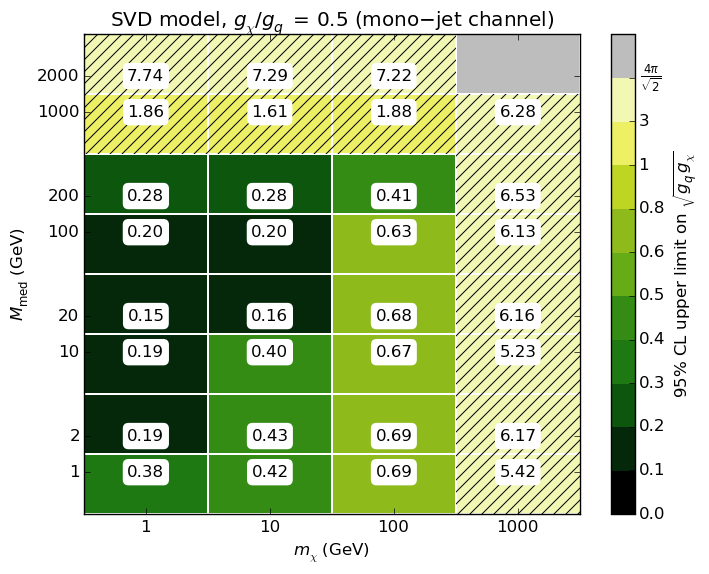
\includegraphics[width=1.\textwidth]{figures/grid_basepoints_SVD_rat05_monojet.png}
      \caption{}
    \end{subfigure}
    \begin{subfigure}[t]{0.45\textwidth}
      \centering
      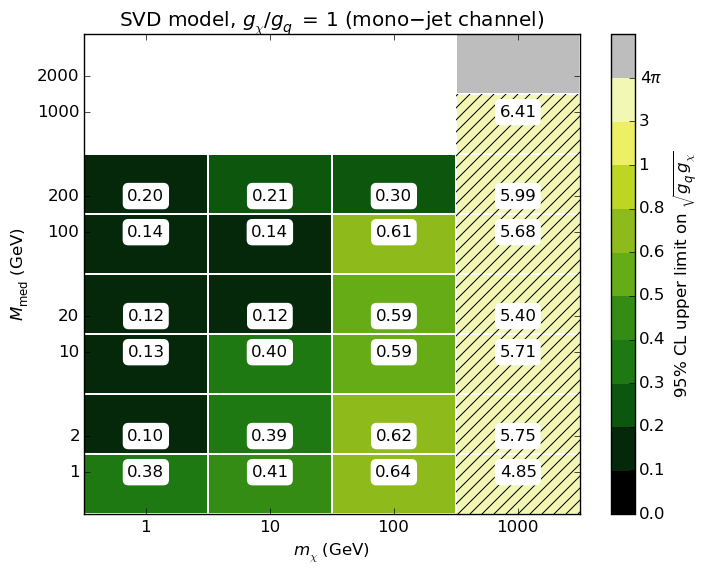
\includegraphics[width=1.\textwidth]{figures/grid_basepoints_SVD_rat1_monojet.png}
      \caption{}
    \end{subfigure}
    \begin{subfigure}[t]{0.45\textwidth}
      \centering
      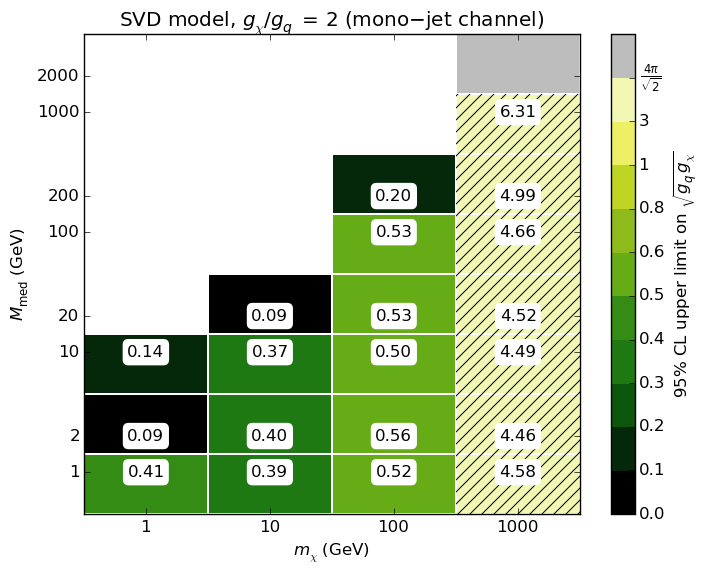
\includegraphics[width=1.\textwidth]{figures/grid_basepoints_SVD_rat2_monojet.png}
      \caption{}
    \end{subfigure}
    \begin{subfigure}[t]{0.45\textwidth}
      \centering
      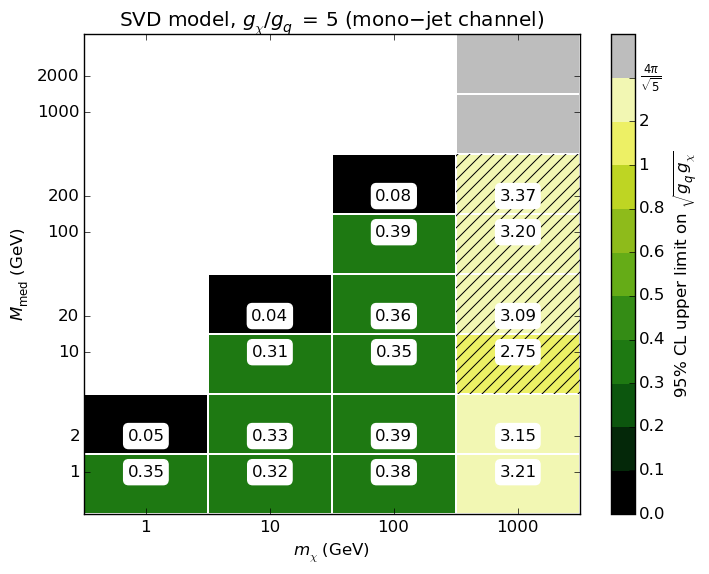
\includegraphics[width=1.\textwidth]{figures/grid_basepoints_SVD_rat5_monojet.png}
      \caption{}
    \end{subfigure}
    \caption{Upper limits on the coupling for the sV model, in the mono-jet channel, for $g_{\chi} / g_q$ = 0.5 (a), 1 (b), 2 (c) and 5 (d). The grey region represents the phase space where no meaningful limit was obtained. The hatched region represents a limit which leads to a width greater than $\Mmed / 2$, so the validity of the calculation begins to fail.}
    \label{fig:Monojet_SVD_couplinglimit}
\end{figure}

\begin{figure}[h]
  \centering
    \begin{subfigure}[t]{0.45\textwidth}
      \centering
      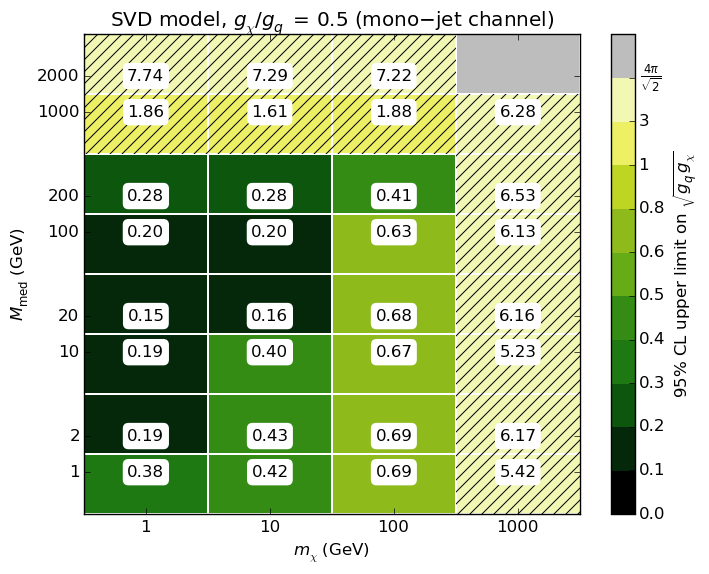
\includegraphics[width=1.\textwidth]{figures/grid_basepoints_SVD_rat05_monojet.png}
      \caption{}
    \end{subfigure}
    \begin{subfigure}[t]{0.45\textwidth}
      \centering
      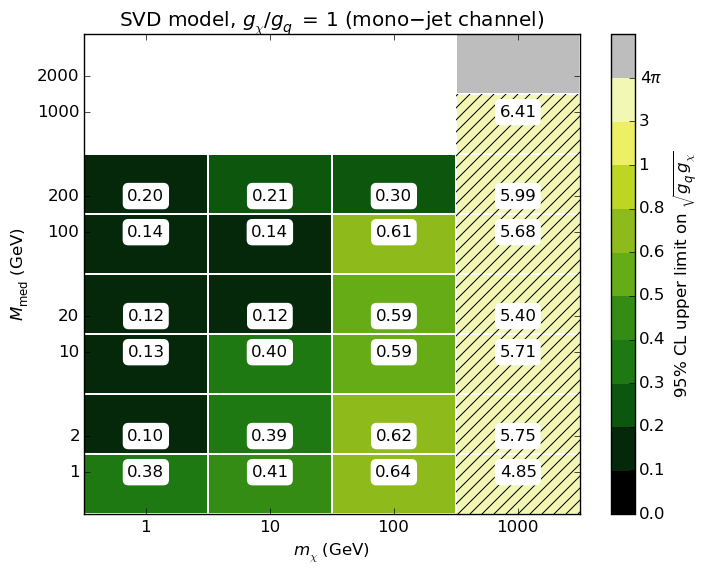
\includegraphics[width=1.\textwidth]{figures/grid_basepoints_SVD_rat1_monojet.png}
      \caption{}
    \end{subfigure}
    \begin{subfigure}[t]{0.45\textwidth}
      \centering
      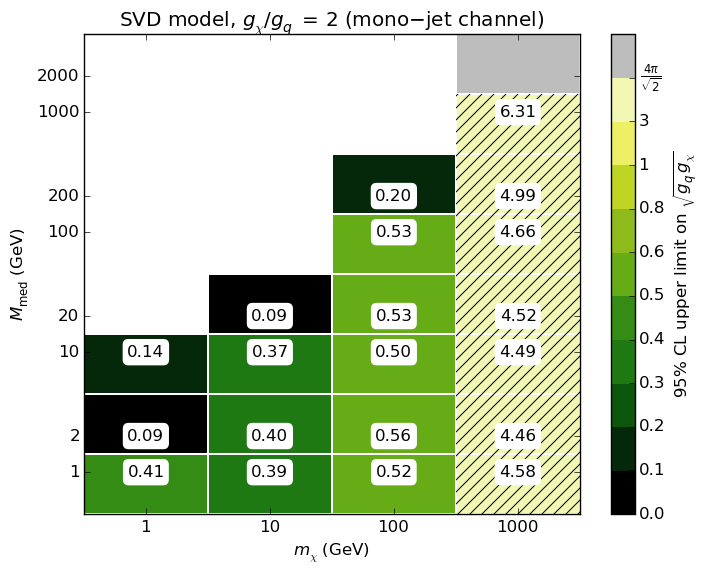
\includegraphics[width=1.\textwidth]{figures/grid_basepoints_SVD_rat2_monojet.png}
      \caption{}
    \end{subfigure}
    \begin{subfigure}[t]{0.45\textwidth}
      \centering
      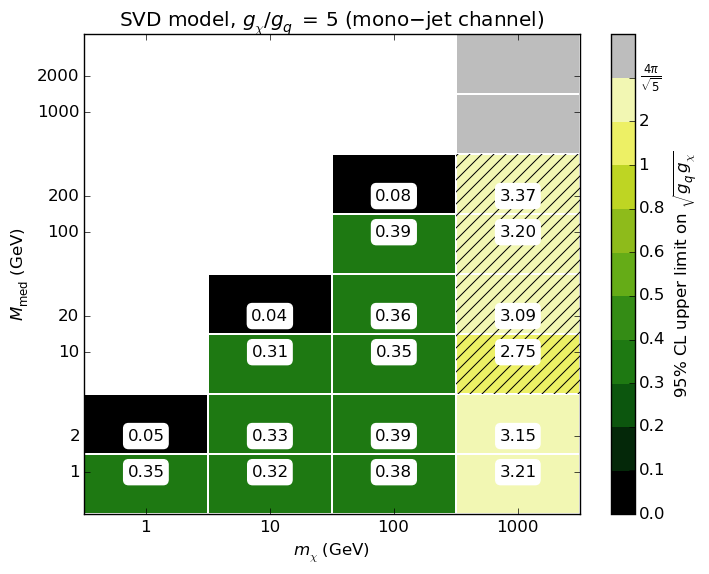
\includegraphics[width=1.\textwidth]{figures/grid_basepoints_SVD_rat5_monojet.png}
      \caption{}
    \end{subfigure}
    \caption{Upper limits on the coupling for the sA model, in the mono-jet channel, for $g_{\chi} / g_q$ = 0.5 (a), 1 (b), 2 (c) and 5 (d). The grey region represents the phase space where no meaningful limit was obtained. The hatched region represents a limit which leads to a width greater than $\Mmed / 2$, so the validity of the calculation begins to fail. TO BE UPDATED WITH sA PLOTS.}
    \label{fig:Monojet_SVD_couplinglimit}
\end{figure}

Results discussion here.

\subsection{Mono-$Z$ channel}

\begin{figure}[h]
  \centering
    \begin{subfigure}[t]{0.45\textwidth}
      \centering
      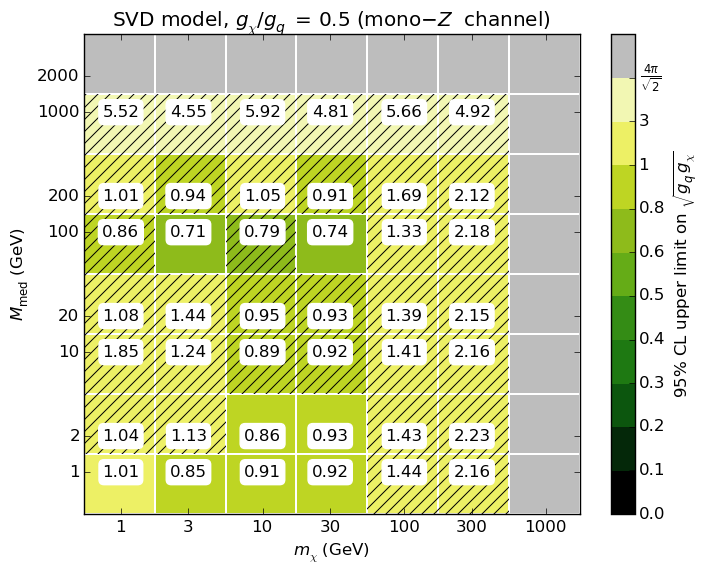
\includegraphics[width=1.\textwidth]{figures/grid_allpoints_SVD_rat05.png}
      \caption{}
    \end{subfigure}
    \begin{subfigure}[t]{0.45\textwidth}
      \centering
      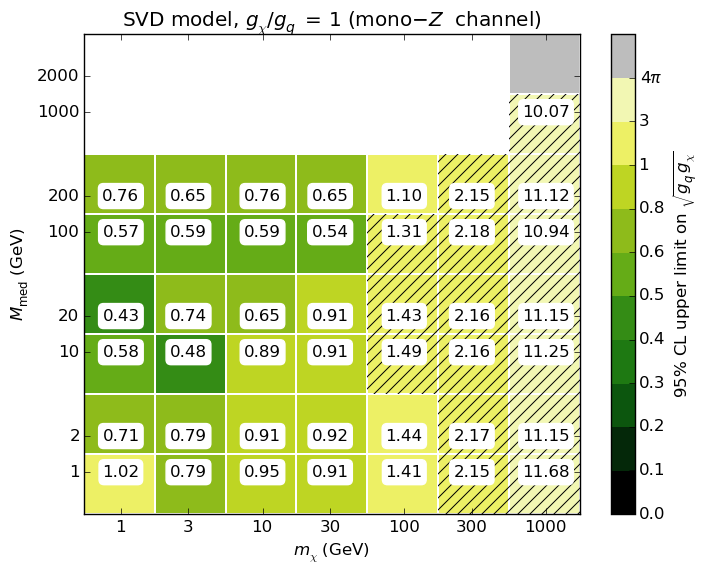
\includegraphics[width=1.\textwidth]{figures/grid_allpoints_SVD_rat1.png}
      \caption{}
    \end{subfigure}
    \begin{subfigure}[t]{0.45\textwidth}
      \centering
      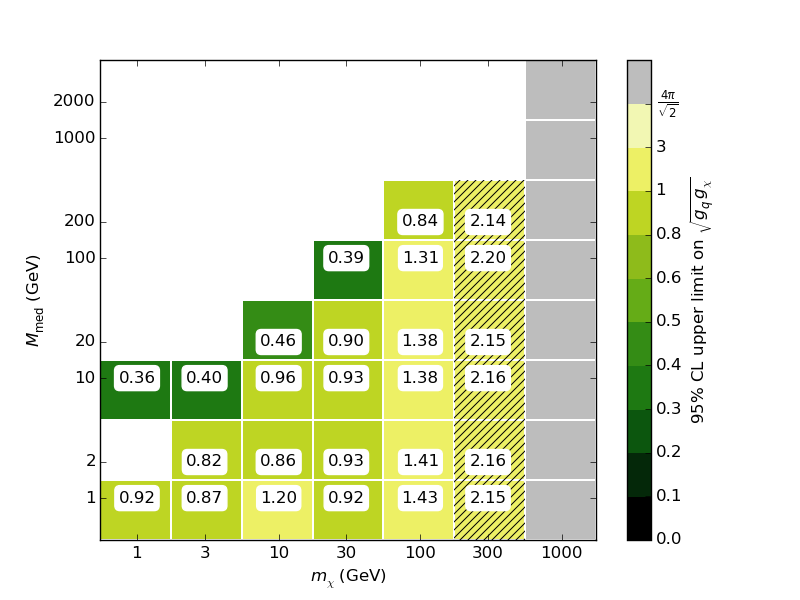
\includegraphics[width=1.\textwidth]{figures/grid_allpoints_SVD_rat2.png}
      \caption{}
    \end{subfigure}
    \begin{subfigure}[t]{0.45\textwidth}
      \centering
      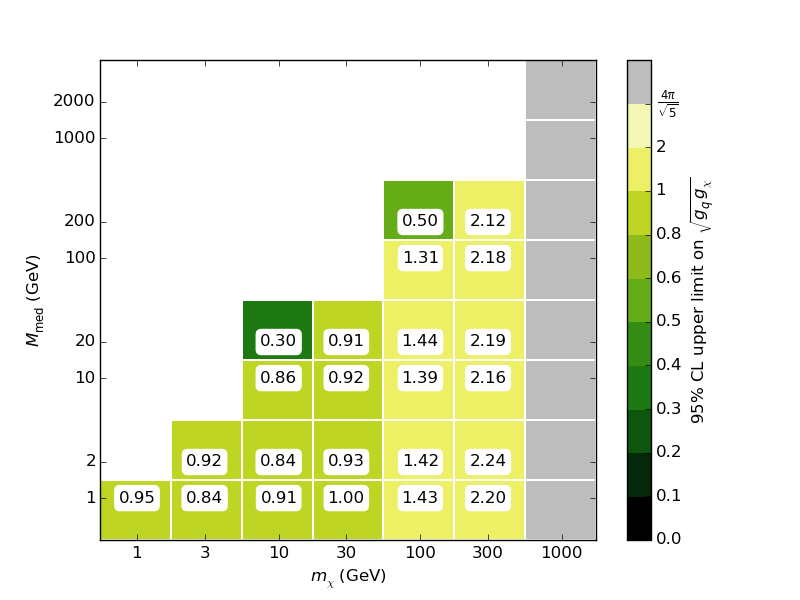
\includegraphics[width=1.\textwidth]{figures/grid_allpoints_SVD_rat5.png}
      \caption{}
    \end{subfigure}
    \caption{Upper limits on the coupling for the sV model, in the mono-$Z$ channel, for $g_{\chi} / g_q$ = 0.5 (a), 1 (b), 2 (c) and 5 (d). The grey region represents the phase space where no meaningful limit was obtained. The hatched region represents a limit which leads to a width greater than $\Mmed / 2$, so the validity of the calculation begins to fail.}
    \label{fig:MonoZ_SVD_couplinglimit}
\end{figure}

\begin{figure}[h]
  \centering
    \begin{subfigure}[t]{0.45\textwidth}
      \centering
      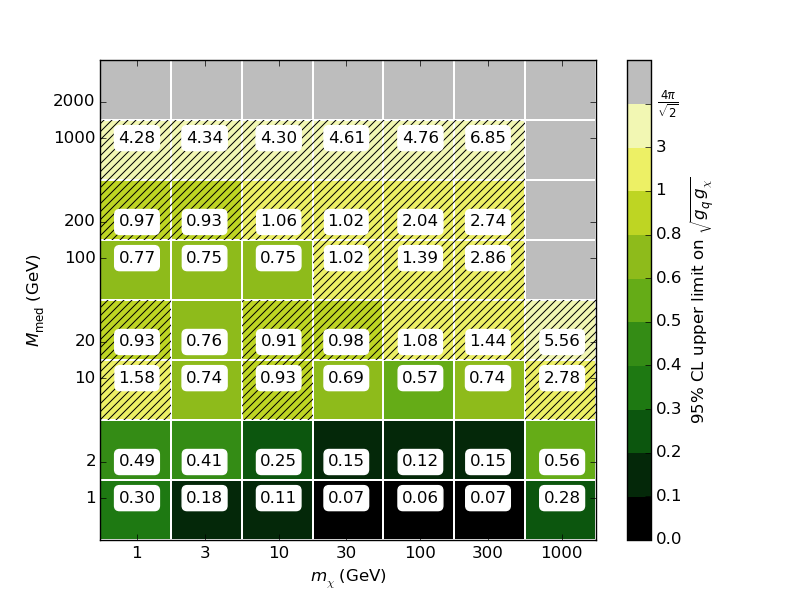
\includegraphics[width=1.\textwidth]{figures/grid_allpoints_SAD_rat05.png}
      \caption{}
    \end{subfigure}
    \begin{subfigure}[t]{0.45\textwidth}
      \centering
      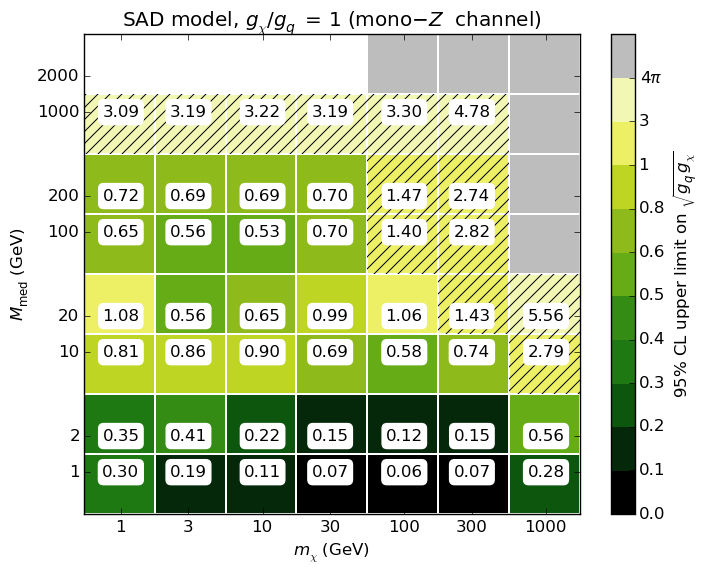
\includegraphics[width=1.\textwidth]{figures/grid_allpoints_SAD_rat1.png}
      \caption{}
    \end{subfigure}
    \begin{subfigure}[t]{0.45\textwidth}
      \centering
      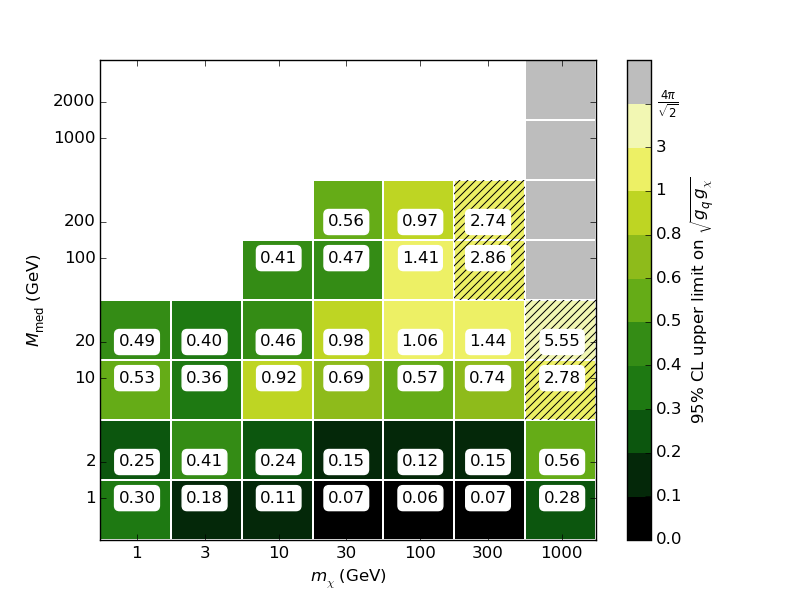
\includegraphics[width=1.\textwidth]{figures/grid_allpoints_SAD_rat2.png}
      \caption{}
    \end{subfigure}
    \begin{subfigure}[t]{0.45\textwidth}
      \centering
      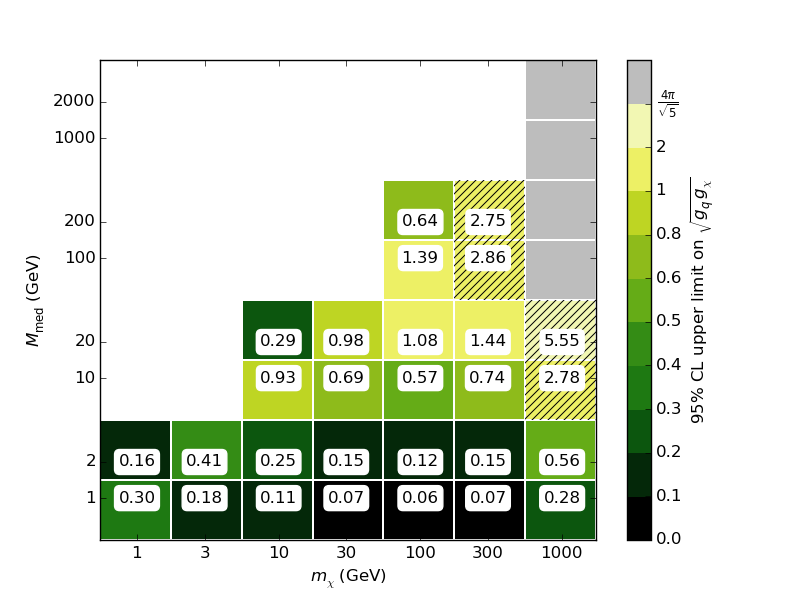
\includegraphics[width=1.\textwidth]{figures/grid_allpoints_SAD_rat5.png}
      \caption{}
    \end{subfigure}
    \caption{Upper limits on the coupling for the sA model, in the mono-$Z$ channel, for $g_{\chi} / g_q$ = 0.5 (a), 1 (b), 2 (c) and 5 (d). The grey region represents the phase space where no meaningful limit was obtained. The hatched region represents a limit which leads to a width greater than $\Mmed / 2$, so the validity of the calculation begins to fail.}
    \label{fig:MonoZ_SAD_couplinglimit}
\end{figure}

\begin{figure}[h]
  \centering
    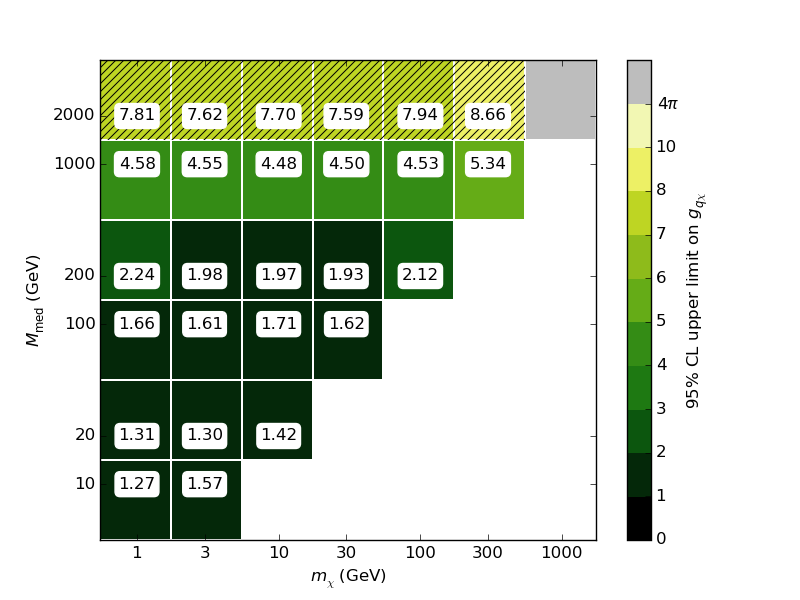
\includegraphics[width=0.6\textwidth]{figures/grid_allpoints_TSD_rat1.png}
    \caption{Upper limit on the coupling $g_{q \chi}$ for the tS model, in the mono-$Z$ channel. The grey region represents the phase space where no meaningful limit was obtained. The hatched region represents a limit which leads to a width greater than $\Mmed / 2$, so the validity of the calculation begins to fail.}
    \label{fig:MonoZ_TSD_couplinglimit}
\end{figure}

Mono-Z limits discussion here. Overall uncertainty on $\sqrt{g_q g_{\chi}}$ generally $ < 10\%$, up to 80$\%$.

\subsection{Mono-$W/Z$ channel}

\begin{figure}[h]
  \centering
    \begin{subfigure}[t]{0.45\textwidth}
      \centering
      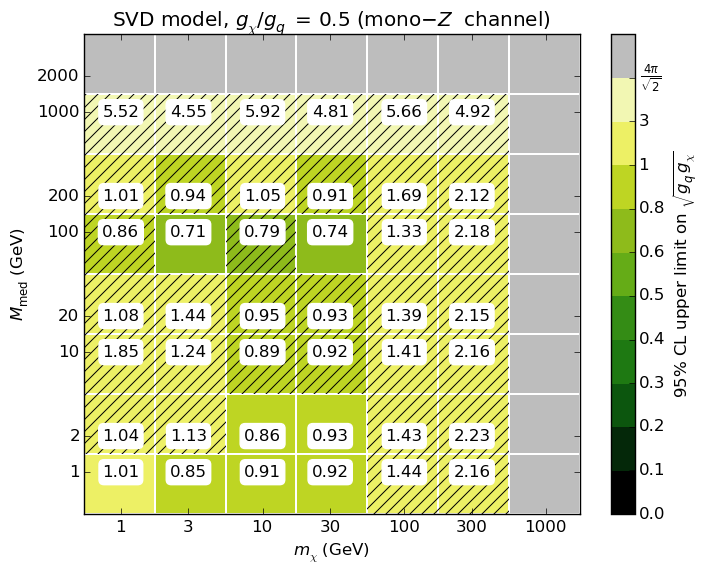
\includegraphics[width=1.\textwidth]{figures/grid_allpoints_SVD_rat05.png}
      \caption{}
    \end{subfigure}
    \begin{subfigure}[t]{0.45\textwidth}
      \centering
      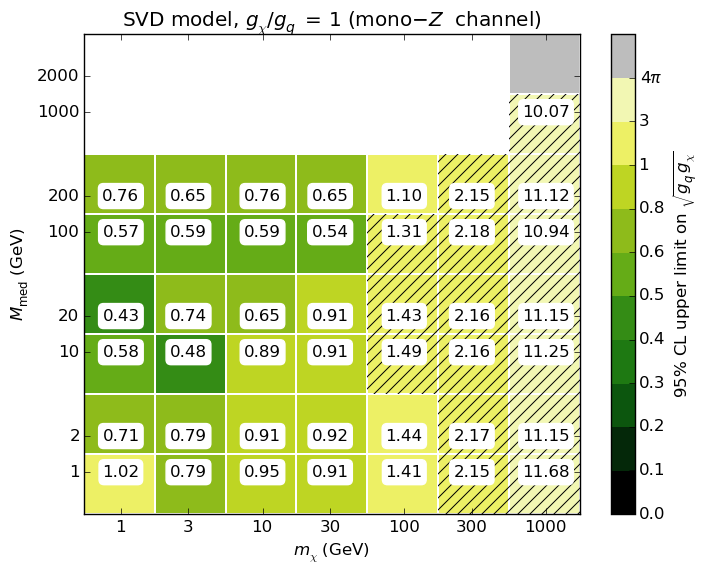
\includegraphics[width=1.\textwidth]{figures/grid_allpoints_SVD_rat1.png}
      \caption{}
    \end{subfigure}
    \begin{subfigure}[t]{0.45\textwidth}
      \centering
      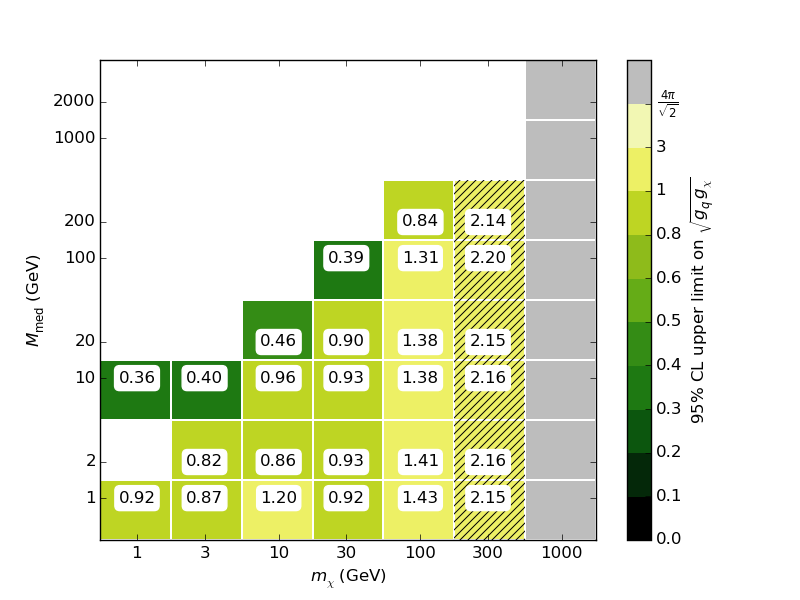
\includegraphics[width=1.\textwidth]{figures/grid_allpoints_SVD_rat2.png}
      \caption{}
    \end{subfigure}
    \begin{subfigure}[t]{0.45\textwidth}
      \centering
      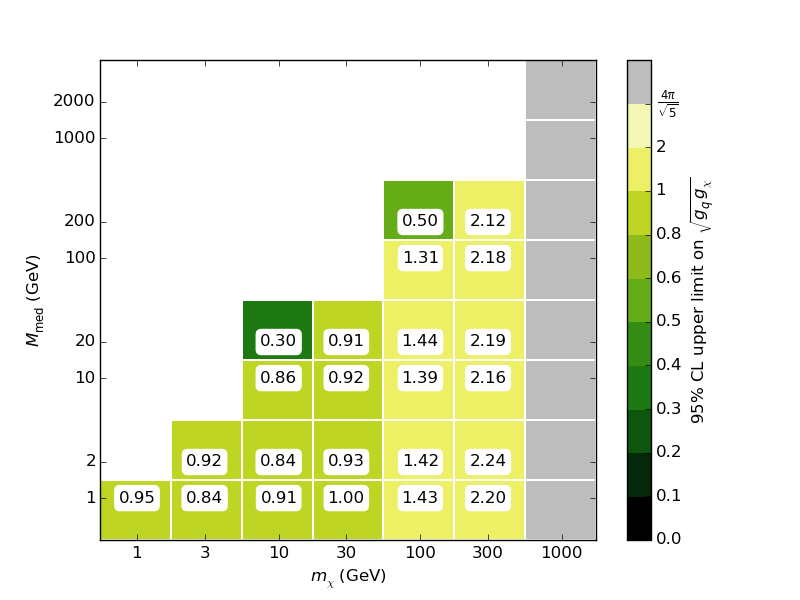
\includegraphics[width=1.\textwidth]{figures/grid_allpoints_SVD_rat5.png}
      \caption{}
    \end{subfigure}
    \caption{Upper limits on the coupling for the sV model, in the mono-$W/Z$ channel, for $g_{\chi} / g_q$ = 0.5 (a), 1 (b), 2 (c) and 5 (d). The grey region represents the phase space where no meaningful limit was obtained. The hatched region represents a limit which leads to a width greater than $\Mmed / 2$, so the validity of the calculation begins to fail. TO BE UPDATED WITH MONOWZ PLOTS.}
    \label{fig:MonoWZ_SVD_couplinglimit}
\end{figure}

\begin{figure}[h]
  \centering
    \begin{subfigure}[t]{0.45\textwidth}
      \centering
      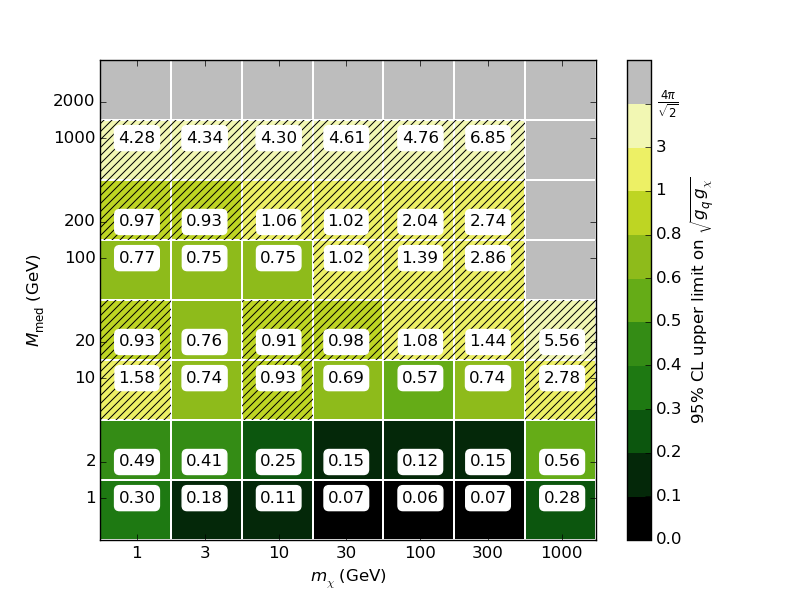
\includegraphics[width=1.\textwidth]{figures/grid_allpoints_SAD_rat05.png}
      \caption{}
    \end{subfigure}
    \begin{subfigure}[t]{0.45\textwidth}
      \centering
      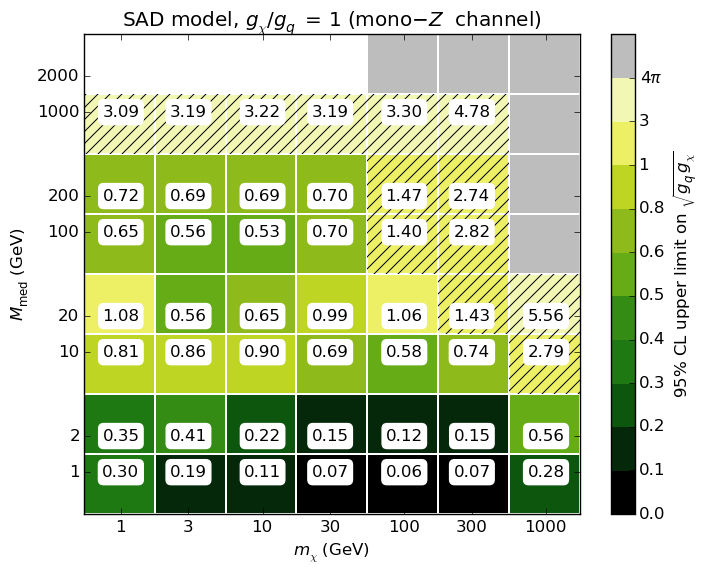
\includegraphics[width=1.\textwidth]{figures/grid_allpoints_SAD_rat1.png}
      \caption{}
    \end{subfigure}
    \begin{subfigure}[t]{0.45\textwidth}
      \centering
      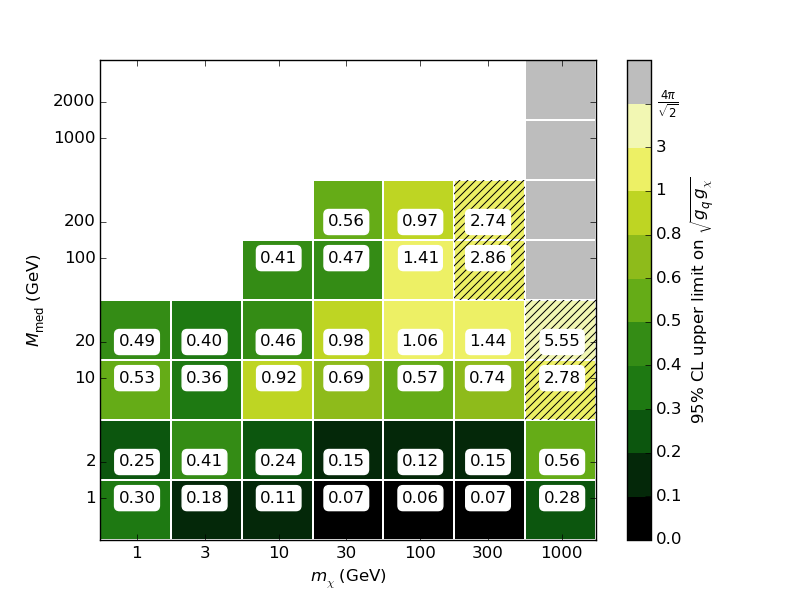
\includegraphics[width=1.\textwidth]{figures/grid_allpoints_SAD_rat2.png}
      \caption{}
    \end{subfigure}
    \begin{subfigure}[t]{0.45\textwidth}
      \centering
      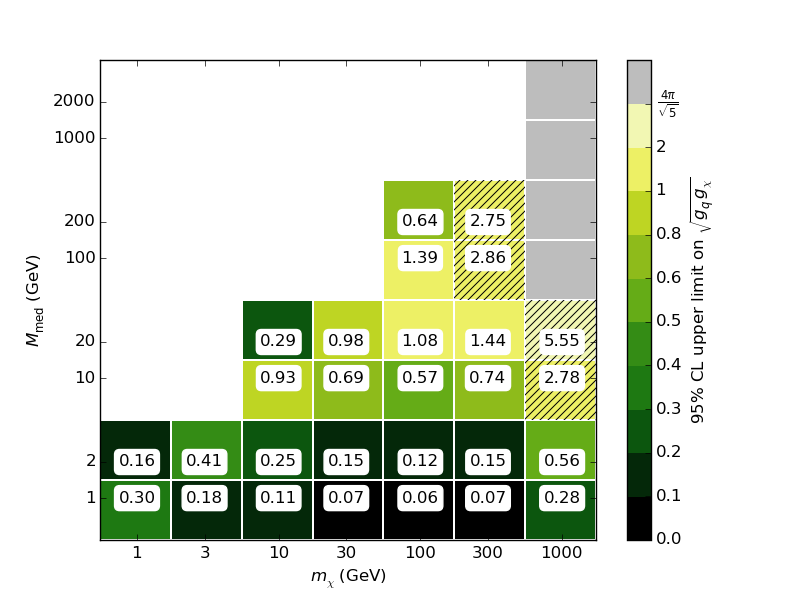
\includegraphics[width=1.\textwidth]{figures/grid_allpoints_SAD_rat5.png}
      \caption{}
    \end{subfigure}
    \caption{Upper limits on the coupling for the sA model, in the mono-$W/Z$ channel, for $g_{\chi} / g_q$ = 0.5 (a), 1 (b), 2 (c) and 5 (d). The grey region represents the phase space where no meaningful limit was obtained. The hatched region represents a limit which leads to a width greater than $\Mmed / 2$, so the validity of the calculation begins to fail. TO BE UPDATED WITH MONOWZ PLOTS.}
    \label{fig:MonoWZ_SAD_couplinglimit}
\end{figure}

\begin{figure}[!h]
  \centering
    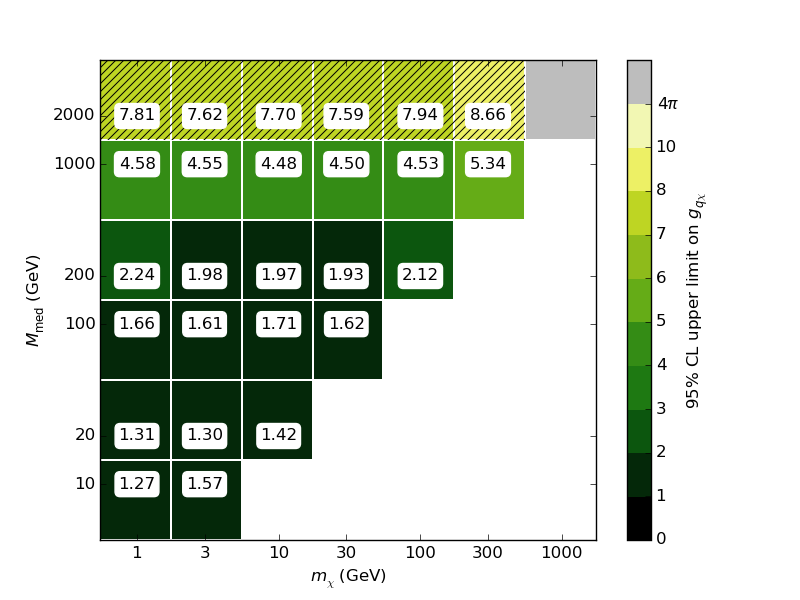
\includegraphics[width=0.6\textwidth]{figures/grid_allpoints_TSD_rat1.png}
    \caption{Upper limit on the coupling $g_{q \chi}$ for the tS model, in the mono-$W/Z$ channel. The grey region represents the phase space where no meaningful limit was obtained. The hatched region represents a limit which leads to a width greater than $\Mmed / 2$, so the validity of the calculation begins to fail. TO BE UPDATED WITH MONOWZ PLOTS.}
    \label{fig:MonoWZ_TSD_couplinglimit}
\end{figure}

Mono-W/Z limits discussion here.

%%%%%%%%%%%%%%%%%%%%%%%%%%%%%%%%
\subsection{Comparison with Relic Density Constraints}
%%%%%%%%%%%%%%%%%%%%%%%%%%%%%%%%

%\comm{Copied from my paper with Karl, so I'll have to rewrite - Tom.}

If dark matter was produced thermally in the early universe, there is a simple relationship between the thermally averaged dark matter self-annihilation cross section $\langle\sigma v\rangle_{\rm ann}$, and the observed relic abundance $\Omega_{\rm DM}h^2$. For a given model, this allows us to find the coupling strength which provides the correct relic abundance as a function of $(m_\chi, M)$.
%
This scenario is by no means a certainty; if the observed dark matter was produced through some mechanism other than thermal production, or if some new physics has an effect on the connection between the self-annihilation rate and the abundance at freezeout, this relationship breaks down. At the same time, thermal dark matter is a well-motivated scenario, and is a useful way to get a sense of the regions of parameter space within which we expect the gravitationally-observed DM to lie.

The observed relic abundance can be approximated as
%
\begin{equation}
  \Omega_{\rm DM}h^2\simeq \frac{2\times2.4\times 10^{-10}\,{\rm GeV}^{-2}}{\langle\sigma v\rangle_{\rm ann}}.
  \label{simplerelic}
\end{equation}
%
Combined with Planck constraints of $\Omega_{\rm DM}^{\rm obs}h^2=0.1199\pm0.0027$ \cite{Ade:2013zuv}, we see that $\langle\sigma v\rangle_{\rm ann}\simeq 4.0\times 10^{-9}\,{\rm GeV}^{-2}$ for thermal relic DM.
%
We use a more accurate method to constrain $\langle\sigma v\rangle_{\rm ann}$, by simultaneously solving an expression for the freezeout temperature as a function of $\langle\sigma v\rangle_{\rm ann}$, and the relic abundance as a function of both $\langle\sigma v\rangle_{\rm ann}$ and the freezeout temperature. We follow the formalism and technique from Ref.~\cite{Busoni:2014gta}.

We indicate on the figures below a line where the LHC constraint on the coupling strength corresponds to the coupling strength which would give thermal relic DM. In regions \draft{above the line or possibly below} this line, the relic density will naively be too large. For DM to lie in this region, either the thermal relic scenario must break down, or the DM annihilates via additional channels not considered here.

\subsection{Comparison with Direct Detection Constraints}
